\section{Introduction}
GPGPU (General-purpose computing on graphics processing units) has been on the rise, due to limitation for CPU's, such as power limitation, and the fact that the computational potential of GPU's (Graphical processing unit) is vastly greater than CPU's, see Figure \ref{potential}. There are technical/physical issue in reaching this potential, for example memory bandwidth, but there is also the conceptual issue of how to map parallelism to parallel hardware.
\begin{figure}[h]
	\centering
	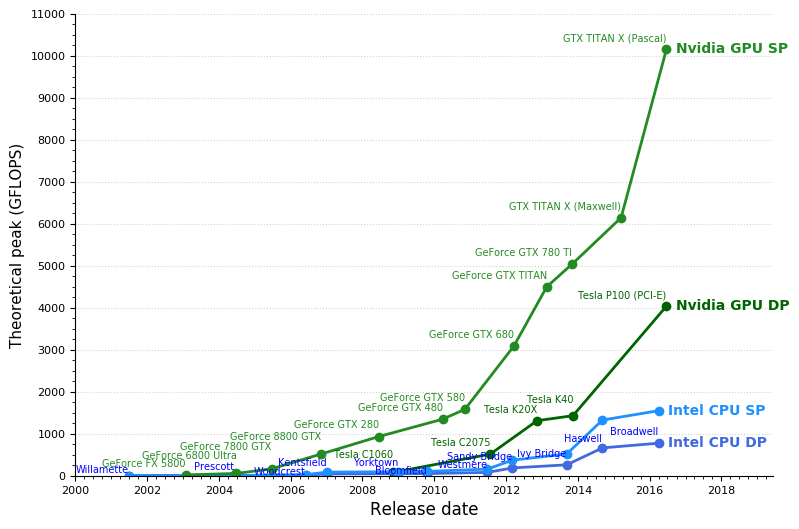
\includegraphics[width=.8\textwidth]{resources/graf.png}
	\caption{A graph showing the computational potential of CPUs and GPUs from 2000---2016 \cite{cpu-vs-gpu}}
	\label{potential}
\end{figure}
In this paper we will implement an autotuner for the programming language Futhark \cite{futhark-home}. Futhark is a programming language that shifts the burden of writing efficient parallel code, from the programmer, to the compiler. It does this by adopting common semantics and syntax from the functional programming paradigm.

However mapping, effectively, functional code, to efficient parallel code, is difficult. Futhark does this by certain rules, these are conceptually similar to \textit{flattening} \cite{flat}, and is dubbed \textit{moderate flattening} \cite{futhark-nested-para}. While this approach was good, a pivotal element for achieving good performance in GPGPU, is to optimize for specific hardware, which moderate flattening did not do (neither does GPU languages such as CUDA or OpenCL, this is left to the programmer). To address this issue, the concept, and implementation, of \textit{incremental flattening} was developed. The concept is that Futhark will generate every distinct possible way of executing a program, these different executions are discriminated, at runtime, based on parameters passed to the program, these parameters symbolizes the amount of parallelism that the hardware executing the program possesses. The process of selection appropriate parameters, for the hardware, is called autotuning, which is what this paper implements.